\documentclass[conference]{IEEEtran}

\usepackage{graphicx}
\graphicspath{{figures/}}
\DeclareGraphicsExtensions{.pdf,.jpeg,.png}

\usepackage[cmex10]{amsmath}
\usepackage{array}
\usepackage{subfig}
\usepackage{url}
\usepackage{booktabs}
\usepackage{sparklines}
\usepackage{tabularx}
\usepackage{verbatim}
\usepackage{listings}
\usepackage{framed}

\usepackage{zi4}

\usepackage{tikz}
\usetikzlibrary{arrows}
\usetikzlibrary{tikzmark}
\usetikzlibrary{calc}
\usetikzlibrary{positioning,fit,backgrounds,decorations.pathmorphing}
\usetikzlibrary{intersections}
\usetikzlibrary{shapes}


% *** Do not adjust lengths that control margins, column widths, etc. ***
% *** Do not use packages that alter fonts (such as pslatex).         ***
% There should be no need to do such things with IEEEtran.cls V1.6 and later.
% (Unless specifically asked to do so by the journal or conference you plan
% to submit to, of course. )


% correct bad hyphenation here
%\hyphenation{op-tical net-works semi-conduc-tor}


\begin{document}
%
% paper title
% can use linebreaks \\ within to get better formatting as desired
\title{How Developers Reason about Error Messages:\\Evaluating Correctly Incorrect Programs}


% author names and affiliations
% use a multiple column layout for up to three different
% affiliations
\author{\IEEEauthorblockN{Titus Barik, Kevin Lubick, Samuel Christie, and Emerson Murphy-Hill}
\IEEEauthorblockA{Computer Science Department\\
North Carolina State University, USA\\
tbarik@ncsu.edu, kjlubick@ncsu.edu, schrist@ncsu.edu, emerson@csc.ncsu.edu}
}

% conference papers do not typically use \thanks and this command
% is locked out in conference mode. If really needed, such as for
% the acknowledgment of grants, issue a \IEEEoverridecommandlockouts
% after \documentclass

% for over three affiliations, or if they all won't fit within the width
% of the page, use this alternative format:
% 
%\author{\IEEEauthorblockN{Michael Shell\IEEEauthorrefmark{1},
%Homer Simpson\IEEEauthorrefmark{2},
%James Kirk\IEEEauthorrefmark{3}, 
%Montgomery Scott\IEEEauthorrefmark{3} and
%Eldon Tyrell\IEEEauthorrefmark{4}}
%\IEEEauthorblockA{\IEEEauthorrefmark{1}School of Electrical and Computer Engineering\\
%Georgia Institute of Technology,
%Atlanta, Georgia 30332--0250\\ Email: see http://www.michaelshell.org/contact.html}
%\IEEEauthorblockA{\IEEEauthorrefmark{2}Twentieth Century Fox, Springfield, USA\\
%Email: homer@thesimpsons.com}
%\IEEEauthorblockA{\IEEEauthorrefmark{3}Starfleet Academy, San Francisco, California 96678-2391\\
%Telephone: (800) 555--1212, Fax: (888) 555--1212}
%\IEEEauthorblockA{\IEEEauthorrefmark{4}Tyrell Inc., 123 Replicant Street, Los Angeles, California 90210--4321}}


% use for special paper notices
%\IEEEspecialpapernotice{(Invited Paper)}


% make the title area
\maketitle


\begin{abstract}
Visual annotations, such as red wavy underlines, are overlaid on source code listings in modern integrated development environments to present compiler errors. Such visual annotations are indicative, but low-fidelity: they offer the developer the line and location of the compiler error notification but do not provide explanation for the underlying causes of the compiler error. Consequently, developers must complex mental models of the errors during error the understanding and resolution. process. Our work proposes a set of expressive visual annotations that assist developers in understanding the underlying compiler error messages. We conducted a study with 28 undergraduate students in software engineering. The results of our demonstrate that even simple visual annotations can aid developers in self-explanation, and allow developers to provide better explanations to others when describing compiler error messages.  Through a cognitive dimensions survey, participants report that our visualizations significantly reduce hidden dependencies as well as hard mental operations needed by the developer.
\end{abstract}
% IEEEtran.cls defaults to using nonbold math in the Abstract.
% This preserves the distinction between vectors and scalars. However,
% if the conference you are submitting to favors bold math in the abstract,
% then you can use LaTeX's standard command \boldmath at the very start
% of the abstract to achieve this. Many IEEE journals/conferences frown on
% math in the abstract anyway.

% no keywords


% For peer review papers, you can put extra information on the cover
% page as needed:
% \ifCLASSOPTIONpeerreview
% \begin{center} \bfseries EDICS Category: 3-BBND \end{center}
% \fi
%
% For peerreview papers, this IEEEtran command inserts a page break and
% creates the second title. It will be ignored for other modes.
\IEEEpeerreviewmaketitle

\section{Introduction}
% no \IEEEPARstart

~\cite{Ko2005} -- bucketing what caused the error
~\cite{Moody2009a}
~\cite{Traver2010}
~\cite{Shneiderman1977}
~\cite{Green1996}

Describe the problem
State your contributions

Here is the problem
It's an unsolved problem
Here is my idea
My ide aworks
Here's how it compares to other approaches

We want computers to explain error notificaitons in the way the humans can best understand them.

Imagine Daena, a software engineer at a medium-sized company.  On a regular basis, she runs into error messages like those shown in Figure 1.  

There is a large body of work that say error messages are confusing [cite sources, like the one with a code snippet sample], but very few go into the why they are confusing [cite paper on message length].  This paper is a part of the latter group.


RQ 1: What are mental models that programmers currently use to understand error notifications?

RQ 2: If programmers are shown a visualization that more closely aligns with their mental models, do they understand the error message better?

RQ 3: How does a mental-model approach of visualization affect developer self efficacy?

We hypothesize that the visual aspect 

The way computers show error notifications is not the same way the humans explain errors to each others.  This suggests to us that there is a misalignment between the computer explanation and human understanding.  We propose the Golden Rule of Error Notifications: Explain onto others as you would want to be explained.  Rather than have humans learn the computers explanation, we want computers to adopt humans' explanations.


I hypothesize this a problem.

Squiggly lines use the same notations to express different types of problems. But errors typically have many hidden dependencies, for example, a default constructor.

Blue.java -> enclosing instance
Invoice -> variable arguments; double methods
kite -> kite default constructor
Quartz generics ->  double int
wilderness -> qualified new of static

system is already visual overlays. provide a position and a location to start with. rough scope. improve on that visual overlays by tackling these other things: cognitive dimensions; physics of notation.

what does this notation look like? pilot study. second study.

self-explanation; disgrams promote self-explanation. developers have to explain it to themselves.

Cognitive dimensions or something else CogSci


\section{Motivating Example}

\lstdefinestyle{JavaError}{
  basicstyle=\small\ttfamily,
}

% BEGIN MELON FIGURE
% ==================
\newsavebox{\melonlisting}
\begin{lrbox}{\melonlisting}
\begin{lstlisting}[style=JavaError]
Melon.java:7: error: 
   variable i might not have been initialized
    }
    ^
1 error
\end{lstlisting}
\end{lrbox}

\begin{figure}[!t]
  \centering
  \subfloat[Melon Wavy\label{fig:melon:base}]
    {\includegraphics{melon_wavy_crop}}
  \\
  % \vspace{0.2cm}
  \subfloat[Melon Expressive\label{fig:melon:explanatory}]
    {\includegraphics{melon_explain_crop}}
  \\
  \subfloat[Melon Error\label{fig:melon:text}]{\usebox{\melonlisting}}
  \caption{A comparison of (a) traditional error notifications and (b) explanatory error notifications in IDEs. Expressive representations are enabled by exposing compilers internals for use by the IDE. TODO: Add line numbers back to the figure.\label{fig:melon}}
\end{figure}

Yoonki is an experienced C++ developer who has recently transitioned to a project that is being developed in the Java programming language. While programming, he encounters a wavy red underline visualization as shown in Figure~\ref{fig:melon:base}, which indicates an error. The problem seems to be related to \texttt{final int i}, which Yoonki recognized as being roughly similar to the concept of a \texttt{const} variable in C++. Yoonki investigates further and notices the full text of the error in the bottom pane of his IDE (Figure~\ref{fig:melon:text}). 

However, Yoonki is now a bit puzzled. The error message indicates that the variable might not be initialized at Line 7. He chooses to ignore this error message as being incorrect because Line 7 contains only a curly brace, which seems to have nothing to do with his problem. He is comfortable in doing so because in C++, he often received unhelpful error messages.

Yoonki incorrectly convinces himself that the problem is that \texttt{final} variables in Java, like \texttt{const} variables in C++, must be initialized at their point of declaration. Satisfied with his explanation, he rewrites Line 2 to read \texttt{final int i = 3;}. Of course, this then results in a downstream error, as Line 6 now returns \texttt{cannot assign a value to final variable i}. Yoonki realizes that of course a constant cannot be re-assigned, so he deletes the entire conditional statement. Even though the program now compiles, the fix happens to be an incorrect one.

The problem here is that Yoonki has learned a reasonable heuristic for how constant variables work in programming languages, but his heuristic fails in this case. Like C++, Yoonki is correct in that Java \texttt{final} variables can only be assigned once. But unlike C++, \texttt{final} variables in Java can be assigned at a point other than the declaration. Yoonki has experienced what we could call a \textit{knowledge breakdown}. In this case, Yoonki has a confirmation bias about how the system is supposed to work, and this false hypothesis has worked reasonably well for him until now.

This false hypothesis remains uncorrected by the IDE. In his IDE, the red wavy underline can only indicate a single location related to the error. In particular, the IDE is unable to convey that the problem is dependent on several program elements. For example, the error message text and the indicated location is accurate in that after this line the variable might be uninitialized, but the IDE does not have an effective way to indicate how that location relates to the \texttt{final} variable.

In contrast, consider our approach, shown in Figure~\ref{fig:melon:explanatory}. Here, Yoonki does not experience the same knowledge breakdown, because the IDE provides a visual explanation of the problem within his source code. Though Yoonki once again incorrectly assumes that \texttt{final} variables must be initialized at declaration, but the visual system implies that the problem is actually related to control flow. Specifically, the expressive visualization is showing Yoonki that there is a code path in which \texttt{i} is assigned a value (when \texttt{b = true}), and another code path where it is not (when \texttt{b = false}). This time, Yoonki correctly fixes the defect by adding an \texttt{else} statement to the condition, initializing it with an appropriate value in the case when \texttt{b = false}.

\section{Visual Explanations Error Messages}
\label{sec:motivation}

In this section, we describe our approach to providing visual explanations for error messages. We operationalize this tool as a set of paper mockups. We begin with the procedure used to construct mockups for both a control and treatment group. We then present a legend of the elements used in our explanations. Finally, we provide explanation for each of the source code listings.

\subsection{Selection Criteria for Mockups}

For our initial study, we decided to use undergraduate students because they are readily available and because we wanted to reserve our more limited industry participants for a full implementation. Because our University requires students to have knowledge of the Java, we selected the language for our visualization system.

Pragmatically, we wanted to keep our entire study under an hour, and due to this experimental design constraint could only present six novel visualizations to participants. We readily admit that the selection of these visualizations was not random, and offer our justification for this decision here. 

We selected our compiler error examples from the OpenJDK diagnostics framework.\footnote{The framework contains a sample source code listing for almost every compiler error within Java. The source files may be downloaded at \url{http://hg.openjdk.java.net/jdk7/tl/langtools/}, and then by browsing to \texttt{test/tools/javac/diags/examples/}.} This framework contains a collection of 382 Java code examples, each of which is designed to generate one or more error messages when compiled.

Since some error messages may be more visually expressible than others (for example, ``illegal escape character'' is not particularly suited to expressive visualization), we hand-selected a set of examples that we believed could benefit most from visual annotations. If no significant results could be identified even from this hand-selected set, then it would suggest that a visual annotation system is not worth pursuing for a full implementation.

Furthermore, our visualization system is not intended to teach new concepts; rather, it is intended to aid the developer in understanding how a particular instance of an error message applies to a specific source file. Consequently, we selected examples based on concepts that students were expected to already know, such as constants and variables, exceptions, and classes.

% participants must already know the underlying concepts, though the visual annotations may sometimes force the participant to reconcile their incorrect understanding of the error message when their interpretation conflicts with the visual annotations presented by the tool.

Ultimately, we selected messages that we believed could effectively demonstrate the rich explanatory capability of visualizations, while taking into consideration the capability of the participants. 

\subsection{Mockup Construction Procedure}

Using the 6 selected error message, we constructed a total of 12 mockups -- 6 for the the control group, and one for the treatment group.  The mockups were designed to resemble an IDE --- each page begins with bordered listing of the source code with visual annotations and line numbers, followed by the compiler error message.

The control group mockups were designed by directly translating the red wavy underlines as provided by the IntelliJ IDE. IntelliJ also provides interactive tooltips for each error, which are shown when the developer hovers over an annotated substring. However, we ignored these interactive features since we are specifically interested in contribution of the explanatory capability of the visualizations in isolation. We chose IntelliJ over the Eclipse IDE because it uses the same text error messages as the command-line OpenJDK compiler, and this consistency turns out to be important for our experimental design.

Thus, the starting point is also indicated in green.

\subsection{Visual Annotation Taxonomy}

\begin{table}[!t]
\caption{Error Annotations\label{tab:viztax}}
\centering

\renewcommand{\tabularxcolumn}[1]{m{#1}}
\begin{tabularx}{\columnwidth}{m{0.4in}X}
\toprule
Symbol & Description\\
\midrule

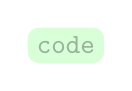
\begin{tikzpicture}
\node[opacity=0.3,fill=green!50,rounded corners,text=black] at (0,0) { \texttt{code} } ;
\end{tikzpicture} 
& Indicates the starting location of the error.\\\\

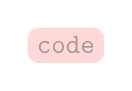
\begin{tikzpicture}
 \node[fill opacity=0.3,fill=red!50,rounded corners] 
    at (0,0) { \texttt{code} };
\end{tikzpicture} & Indicates issues related to the error.\\\\

\begin{tikzpicture}
\draw[>=latex,->] (0,0) -| (1em, 1em );
\end{tikzpicture}  & Arrows can be followed. They indicate the next relevant location to check.\\\\


\begin{tikzpicture}
 \node[circle,draw=gray,very
    thin,fill=black,text=white,inner sep=1pt] at (0,0) {\tiny 1};
\end{tikzpicture} & Enumerations are used to number items of potential interest, especially when the information doesn't fit within the source code.\\\\

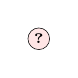
\begin{tikzpicture}
\node (node 1) at (0,0) [circle,draw=gray,very
    thin,fill=red!10,text=white,inner sep=1pt,draw=black,text=black] at (0,0) {\tiny \textbf{?}};
\end{tikzpicture} & The compiler expected an associated item, but cannot find it.\\\\



\begin{tikzpicture}
  \node[draw=red,cross out,inner sep=2pt,fill=black,text=white,thick] at (0,0) {};
\end{tikzpicture} & Indicates a conflict between items.\\\\

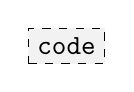
\begin{tikzpicture}
\node[draw,rectangle,draw=black,fill=gray!10,dashed,right] at (0,0) {\texttt{code}};
\end{tikzpicture} & Explanatory code or code generated internally by the compiler. The code is not in the original source.\\\\

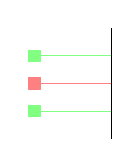
\begin{tikzpicture}
\draw (0,0) -- (0,-4em);
\draw[>=square,->,draw=green!50,fill=green!50]    
      (0,-1em) -- +(-3em, 0em);
  \draw[>=square,->,draw=red!50,fill=red!50]
    (0,-2em) -- +(-3em, 0em);
  \draw[>=square,->,draw=green!50,fill=green!50] 
    (0,-3em) -- +(-3em, 0em); -- +(-3em, 0em);
\end{tikzpicture} & Indicates code coverage. Green lines indicate successfully executed code. Red lines indicate failed or skipped lines.\\

\bottomrule
\end{tabularx}
\end{table}
\renewcommand{\tabularxcolumn}[1]{p{#1}}

Based on our findings from the pilot study (described in Section~\ref{sec:pilotstudy}), we derived a set of 7 visual annotations, and an additional annotation, code coverage, which we did not directly observe but speculated might be useful to developers. Experimentally, we did so in order to determine whether a priming effect was present. These are shown in Table~\ref{tab:viztax}.


\subsection{Explanation of Mockups}

Mockups are 

\textbf{Apple}

\textbf{}

TODO move this before pilot -- we'll make it work, even though it required some forward referencing

% ==================

% BEGIN ZEBRA FIGURE
% ==================
\newsavebox{\zebralisting}
\begin{lrbox}{\zebralisting}
\begin{lstlisting}[style=JavaError]
Zebra.java:8: error: cannot infer type arguments for BlackStripe<>;
   Stripe<String> sf1 = new BlackStripe<>("Marty");
                        ^
  reason: inferred type does not conform to declared bound(s)
    inferred: String
    bound(s): Number
1 error
\end{lstlisting}
\end{lrbox}

\begin{figure*}[!t]
  \centering
  \subfloat[Zebra Wavy]
    {\includegraphics{zebra_wavy_crop}\label{lst:ma:traditional}}
  \\
  \subfloat[Zebra Expressive\label{lst:ma:explanatory}]
    {\includegraphics{zebra_explain_crop}}
  \\
  \subfloat[Zebra Error]{\usebox{\zebralisting}}

  \caption{Zebra\label{lst:ma}}
\end{figure*}
% ==================

\begin{table*}[!t]
\caption{Participant Explanation and Recall Tasks\label{tab:tasks}}
\centering
% Some packages, such as MDW tools, offer better commands for making tables
% than the plain LaTeX2e tabular which is unsolved here.
\begin{tabularx}{\textwidth}{lllX}
\toprule
Task Order & Task Name & OpenJDK File & Error Message\\
\midrule

T1 & Melon & \texttt{VarMightNotHaveBeenInitialized.java} & \texttt{variable i might not have been initialized} \\
[0.2cm]
\midrule

T2 & Kite & \texttt{UnreportedExceptionDefaultConstructor.java} & \texttt{unreported exception Exception in default constructor} \\
[0.2cm]
\midrule

T3 & Brick & \texttt{RefAmbiguous.java} & \texttt{reference to m is ambiguous, both method m(int,double) in Brick and method m(double,int) in Brick match}\\
[0.2cm]
\midrule

T4 & Zebra & \texttt{InferredDoNotConformToBounds.java} & \texttt{cannot infer type arguments for BlackStripe<>;\newline
reason: inferred type does not conform to declared bound(s)\newline\newline
inferred: String\newline
    bound(s): Number}\\
[0.2cm]
\midrule

T5 & Apple & \texttt{RepeatedModifier.java} & \texttt{repeated modifier
}\\
[0.2cm]
\midrule

T6 & Trumpet & \texttt{UnreachableCatch1.java} & \texttt{unreachable catch clause\newline     
  thrown types FileNotFoundException,EOFException have already been caught
}\\
[0.2cm]

\bottomrule
\end{tabularx}
\end{table*}

Our visualizations are simpler, but they are grounded in empirical research, based on how developers actually explained code to us system doesn't actually exist. this is a paper prototyping task. we first had to determine a free-body diagram system. using a pilot study (see section...). Cognitive dimensions used.  

tool tip problem

TODO six examples and explain why we chose them.  Show two visualizations here, contrasted with squiggly versions, and link to all 6 in off-paper url (WITH GOOGLE ADS).


\section{Pilot Study}
\label{sec:pilotstudy}

To seed a set of visual annotations that are appropriate for explaining error messages, we conducted an informal classroom activity with junior level computer science students. Each student was given a sheet of paper with a source code listing and the corresponding compiler error message. The source code listings were unadorned and lacked any visual annotations.

Students were paired in order to perform an explainer-listener active learning exercise. This is an exercise in which one student, the explainer, is asked to verbally explain the error message to the other student, while visually annotating the source code listing during their explanation. Access to external materials was not allowed. After two minutes of explanation, roles were swapped and the second explainer annotated the second error message.

Source code listings were randomly selected from four examples, pulled verbatim from the OpenJDK 7 unit tests for compiler diagnostics framework. The four examples that were used for the pilot study are found in Table~\ref{tab:tasks}, and no students within a pair received the same source code listings. In total, we collected 73 samples and aggregated the types of visualizations present in the set.  17 participants received T1 (23\%), 12 participants received T2 (16\%), 20 students received T3 (27\%), and 24 participants received T6 (33\%). Students did not receive tasks T4 or T5.


\begin{table}[!t]
\caption{Frequency of Visual Annotations in Pilot\label{tab:pilot}}
\centering
\begin{tabularx}{\columnwidth}{lrX}
\toprule
Annotation & Frequency & Description\\
\midrule
Point & 49 & Indicates that a particular token or set of tokens has been marked. Examples include underlining or circles the token(s).\\
Text & 45 & Indicates natural language text. For example, ``assign a value to the variable'' or ``dead code''.\\
Association & 33 & Indicates an association between two or more elements, which is accomplished by drawing a connecting line between the elements, with or without arrow heads.\\
Symbol & 20 & Symbols include visual annotation such as \texttt{?} or \texttt{x}, or numbered circles, to name a few.\\
Code & 14 & Explanatory code that is written in order to explain the error message, for example, \texttt{if (b == false)} or \texttt{m(1.0, 2)}. This does not have to be correct Java code, but should be interpretable as pseudocode.\\
Strikethrough & 5 & The strikethrough is separated from the point annotation, not only because this annotation is provided by IDEs today, but also because strikethrough tends to be resolution-oriented, rather than explanation-oriented.
\\
Multicolor & - & The use of more than a single color to explain a concept. For example, green may be used to indicate lines that are okay, and red to indicate lines that are problematic. This option was not available to students in the pilot study.\\
\bottomrule
\end{tabularx}
\end{table}

From these annotations, we performed two passes over the student responses. In the first pass, we created a taxonomy of visual annotations, whose cardinality was reduced based on common features. We then classified the student responses using this taxonomy. The aggregated results are shown in Table~\ref{tab:pilot}.

Because of the informal nature of this uncontrolled study, we make no further attempt to quantitatively describe this data in additional detail. Of particular interest to us is that, after points and text, students most frequently used associations between text in the source code. This association feature is not available in integrated development environments today.

\section{Experiment}

This section details the design and execution of our experiment. We begin with a description of our participant population, followed by the experimental procedure.

\subsection{Participants}

We recruited 28 participants ($n = 28$) from a third-year undergraduate course in Software Engineering. We offered participants extra credit on their final exam as an incentive for participating in the study. Participants self-reported demographic data. Five of participants were female (17.8\%). The mean age of the participants was 22 ($s = 3.6$). Participants reported a mean of 9 months ($s = 12$) of industry programmer experience. We further identified outliers through quartile construction to find the standard deviation attributable to three participants self-reporting 28 months, 40 months, and 48 months of experience. Without these participants, the mean industry programmer experience is 5 months ($s = 6$). We performed all analyses with and without these outliers. We concluded that the high outliers were otherwise unremarkable except in their self-reporting and therefore we gave no special consideration to them in subsequent reporting within this paper.

Participants predominantly reported using the Eclipse IDE as their primary Java programming environment; two participants reported IntelliJ. On a 4-point Likert-type item scale of \emph{Novice---Expert}, 13 participants reported their overall programming ability as Intermediate (46\%), 14 as Advanced (50\%), and 1 as Expert (4\%). No participants ranked themselves as Novice. On a 4-point scale \emph{Not knowledgeable---Very knowledgeable}, 19 participants indicated they they were knowledgeable about Java (68\%), and the remaining 9 participants indicated that they were very knowledgeable about Java (32\%).

% \subsection{Methodology}

% http://www.real-statistics.com/non-parametric-tests/mann-whitney-test/


% this is a non-random sampling of error messages.

% TODO mention annotating correctness

% How to Report Mann-Whitney U: http://yatani.jp/HCIstats/MannWhitney
% "Median latencies in groups E and C were 153 and 247 ms; the distributions in the two groups differed significantly (Mann–Whitney U = 10.5, n1 = n2 = 8, P < 0.05 two-tailed)."

\subsection{Procedure}

Schnidermann did a study with nonprogrammers and programmers to see if programmers were better able to reproduce code listings, indicating that programmers semantically remember code.  We based our study off of Schnidermann's by designing our study with two secions -- a recognition section and a recall section.

\begin{figure}[!t]
  \centering  
  \subfloat[Command prompt.\label{fig:progenv:cmd}]{\includegraphics[width=\columnwidth]{cmd.png}}\\
  \subfloat[Minimal text editor.\label{fig:progenv:text}]{\includegraphics[width=\columnwidth]{figures/notepad2.png}}  
  \caption{Participants were presented with a command prompt in which they had the \texttt{compile} command available to them.\label{fig:progenv}}
\end{figure}

\textbf{Assignment.}
We randomly assigned participants a participant id and to one of two groups -- control or treatment, such that each group had an equal number of participants.   This resulted in 14 participants per group. The control group received error messages containing only TODO underline the following /TODO wavy red underlines (i.e. squiggly lines) as commonly found in IDEs today.  The treatment group received error messages using the visualization taxonomy outlined in Section \ref{Approach} as well as a legend explaining the novel visualizations.  All other aspects were kept the same, thus any observed differences are attributable to the visualizations used.

\textbf{Consent.}
Before proceeding with the study, participants filled out an IRB consent form and indicated whether or not they wanted their audio to be recorded.  


\textbf{Recording.} 
For participants that agreed to be recorded (N=26), we used desktop recorder software to record both the audio of the explanations as well as screen interactions during Part 2.

\textbf{Part 1 -- Comprehension.}
Participants were given 6 error notifications detailed above and were asked to look at the notifications for 30 seconds.  Then, they were instructed to explain the cause of the errors and to visually annotate a second blank copy of the source code using colored pencils.  This part was procedurally similar to the pilot study detailed in Section \label{PilotStudy}, except the participant always held the role of Explainer.


\subsection{Cognitive Dimensions Survey}
\label{subsec:cogdim}

At this point, a cognitive dimensions survey was administered to the participants CITE CD SURVEY. We picked cognitive dimensions because the participants don't need to be HCI experts to evaluate our visualizations and it was a pre-existing validated survey.  Most cognitive dimensions focus on interaction-based interfaces, so we removed those, leaving us with four dimensions to survey.  There is some literature TODO CITE that cognitive dimensions are still confusing, despite being targeted at non-experts, so we included a positive and a negative example for each, using familiar examples from every day computing.  

The survey we administered is copied below:
\begin{enumerate}
	\item \textbf{Hidden Dependencies}: A hidden dependency is a relationship between two components such that one of them is dependent on the other, but that dependency is not fully visible. For example, Excel spreadsheets often contain cells are referenced from other sheets and so you can’t easily tell if modifying a given cell will or will not have an impact elsewhere (many hidden dependencies). The LabView programming language\footnote{http://www.ni.com/labview/} makes data flow explicit, and so there are fewer hidden dependencies. 
	\emph{On a scale of 1-5, how visible are these dependencies in the annotations you just evaluated?}

	\item \textbf{Consistency}: Things are consistent when similar semantics are expressed in similar syntactic forms, that is, things that look similar either behave similarly or mean similar things. For example, the green triangle that means ``play'' is a nearly universal signal, so it is very consistent. The grammar rules for English have lots of exceptions and irregular words, so they are less consistent.

On a scale of 1-5, how consistent were the annotations you just evaluated?

	\item \textbf{Hard mental operations}: When it feels like you have to juggle many things in your head to keep things straight or to properly use something, that is an indication of hard mental operations. For example, if you had to file your taxes without being able to write anything down except your final amounts, doing taxes would require many hard mental operations. If you use tax-assistant software that keeps track of the intermediate steps for you and makes sure the correct boxes are filled, there are fewer hard mental operations.

On a scale of 1-5, to what extent did the annotations require hard mental operations?

	\item \textbf{Role Expressiveness}: A system with high role expressiveness has an intuitive design and feel - it is easy to tell why the respective design decisions were chosen. For example, a well organized machine shop has all the supplies and tools for a given task in the same spot - painting supplies on one table, cutting machines near each other, drill bits next to the drill, etc. The QWERTY keyboard layout has been criticized for having low role expressiveness because of the scattered keys and a lack of cohesive grouping.

On a scale of 1-5, how was the role expressiveness of the annotations you saw previously?

\end{enumerate}

\subsection{Explanation Rating by Cognitive Breakdown}

huh



\subsection{Recall Task}

The interface used by the participants is shown in Figure~\ref{fig:progenv}.

To get a second measure comprehension, participants were given  a text editor and a command-line compiler to write code that produces each of the six error messages seen in Part 1.  For each notification, participants needed to complete code writing in five minutes or less.

\section{Results}

Here are our results.

\subsection{Visualizations Lead to More Correct Explanations}
\label{subsec:result:explanation}

\begin{figure}[!t]
  \centering
  \subfloat[]
    { \includegraphics[height=2.5in]{P658_melon} }
  \subfloat[\label{fig:partmelon:treatment}]
    {\includegraphics[height=2.5in]{P469_melon}}
  \caption{A contrast between visual explanations offered by (a) control group participant with explanation rating of Fail, and (b) treatment group participant with explanation rating of Excellent. The participant in (a) incorrectly identifies that the variable \texttt{i} must be initialized in the declaration. This in turn leads to a downstream breakdown in that \texttt{final} variables cannot be initialized more than once. The participant in (b) explains how the variable is only sometimes initialized.}
\end{figure}


Our hypothesis was that having visual explanations for compiler error messages would yield more correct explanations by participants. 

To validate this hypothesis, we conducted an inter-rater reliability exercise in which the first and second authors independently rated the participants' explanations, without consideration of group. The first author assigned ratings using both the recorded verbal explanations of the participant as well as their paper markings. The second author assigned ratings using only the paper markings. This was a deliberate design decision to ascertain the extent to which visual markings alone can be used to infer the correctness of an explanation, since actual developers will not have a physical explainer assisting them with understanding error messages.

We assigned ratings to each of the 168 tasks on a Likert-type scale from 1--4, labeled Fail, Poor, Good, and Excellent, respectively. For each task, we developed a rubric for what constituted a correct explanation and noted common misconceptions, as typically done in traditional academic grade assignments. Given the ordinal scale, a weighted Cohen's Kappa for 2 Raters test, using equal weighting for each rating, found moderate agreement between the raters ($n = 168, \kappa = 0.47, p < .001$). Ratings with audio and verbal markings had a median of 3, while verbal markings only had a median of 4, but a paired Wilcoxon Signed-Rank Test did not identity these differences between the two raters as being significant ($n_1 = n_2 = 168, S = 182, p < .25$), Thus, the data suggest that visual markers capture the correctness of the full explanation reasonably well. 

\begin{figure}[!t]
\centering
\includegraphics[width=\columnwidth]{ratingbygroup}
\caption{Explanation rating by group.The treatment group provides significantly higher rated explanations than the control group. TODO: Change the figure labels so that they say Fail, Poor, Good, and Excellent.\label{fig:ratingbygroup}}
\end{figure}

The distribution between the two groups, binned by rating, is shown in Figure~\ref{fig:ratingbygroup}. Between the control and treatment groups, a Wilcoxon Rank-Sum Test confirms that participants gave significantly better explanations in the treatment group ($n_1 = n_2 = 84, Z = 2.23, p = .026)$. 

\subsection{A Visual Taxonomy Elicits More Expressive Visual Explanations}



\begin{figure}[!t]
\centering
\includegraphics[width=\columnwidth]{apple_exp}
\caption{A participant drew this on a piece of paper.\label{fig_sim}}
\end{figure}


\begin{figure}[!t]
\centering
\includegraphics[width=\columnwidth]{annotation_by_group}
\caption{Annotations by group, filled with usage across tasks.}\label{fig:annotationbygroup}
\end{figure}

\begin{table}[!t]
\caption{Number of Features by Task and Group\label{tab:features}}
\centering
\begin{tabular}{lrcrc}
\toprule
& \multicolumn{4}{c}{Number of Features}\\ \cmidrule(lr){2-5}
 & \multicolumn{2}{c}{Control}& \multicolumn{2}{c}{Treatment}\\
 \cmidrule(lr){2-3} \cmidrule(lr){4-5}
 Task & Median & Dist & Median & Dist\\ 
\midrule
T1 & 
2 &
\definecolor{sparkspikecolor}{named}{darkgray}
\begin{sparkline}{4}
\sparkspike .083 .4
\sparkspike .25 1
\sparkspike .417 .6
\sparkspike .583 .2
\sparkspike .75 .2
\end{sparkline}
&
3 &
\definecolor{sparkspikecolor}{named}{olive}
\begin{sparkline}{4}
\sparkspike .083 .2
\sparkspike .25 .4
\sparkspike .417 0.6
\sparkspike .583 0.4
\sparkspike .75 0.01
\end{sparkline}
\\

T2 &
2 & \definecolor{sparkspikecolor}{named}{darkgray}
\begin{sparkline}{4}
\sparkspike .083 .2
\sparkspike .25 1
\sparkspike .417 .6
\sparkspike .583 .01
\sparkspike .75 .01
\end{sparkline}
&
2 & \definecolor{sparkspikecolor}{named}{olive}
\begin{sparkline}{4}
\sparkspike .083 .2
\sparkspike .25 .8
\sparkspike .417 .4
\sparkspike .583 .2
\sparkspike .75 0.01
\end{sparkline}
\\


T3 &
2 & 
\definecolor{sparkspikecolor}{named}{darkgray}
\begin{sparkline}{4}
\sparkspike .083 .17
\sparkspike .25 1
\sparkspike .417 .17
\sparkspike .583 .17
\sparkspike .75 0.01
\end{sparkline}
&
2 &
\definecolor{sparkspikecolor}{named}{olive}
\begin{sparkline}{4}
\sparkspike .083 .17
\sparkspike .25 .83
\sparkspike .417 .33
\sparkspike .583 .33
\sparkspike .75 .01
\end{sparkline}
\\

T4 &
2 & \definecolor{sparkspikecolor}{named}{darkgray}
\begin{sparkline}{4}
\sparkspike .083 .5
\sparkspike .25 .83
\sparkspike .417 0.33
\sparkspike .583 0.5
\sparkspike .75 0.01
\end{sparkline}
&
3 & \definecolor{sparkspikecolor}{named}{olive}
\begin{sparkline}{4}
\sparkspike .083 .33
\sparkspike .25 .33
\sparkspike .417 1
\sparkspike .583 .33
\sparkspike .75 .01
\end{sparkline}
\\

T5 &
1 & \definecolor{sparkspikecolor}{named}{darkgray}
\begin{sparkline}{4}
\sparkspike .083 1
\sparkspike .25 .67
\sparkspike .417 0.17
\sparkspike .583 0.17
\sparkspike .75 0.01
\end{sparkline}
&
2 & \definecolor{sparkspikecolor}{named}{olive}
\begin{sparkline}{4}
\sparkspike .083 .33
\sparkspike .25 .83
\sparkspike .417 .33
\sparkspike .583 .17
\sparkspike .75 .01
\end{sparkline}
\\

T6 &
3 & \definecolor{sparkspikecolor}{named}{darkgray}
\begin{sparkline}{4}
\sparkspike .083 .33
\sparkspike .25 .33
\sparkspike .417 1
\sparkspike .583 0.17
\sparkspike .75 0.01
\end{sparkline}
&
3 & \definecolor{sparkspikecolor}{named}{olive}
\begin{sparkline}{4}
\sparkspike .083 .01
\sparkspike .25 .5
\sparkspike .417 .83
\sparkspike .583 0.33
\sparkspike .75 .01
\end{sparkline}\\
\bottomrule
\end{tabular}
\end{table}

Table~\ref{tab:features} summarizes the number of features used for each task, partitioned by control and treatment groups. We think a quantifiable measure of whether or how expressive is the number of features used in the visualization -- such as associations, points, or symbols. Using a Wilcoxon Rank-Sum Test, we find that there the treatment group using significantly more visual annotations in their explanations than the control group ($n_1 = n_2 = 84Z = 2.15, p = .032)$. 

Figure~\ref{fig:annotationbygroup} shows the distribution of the annotations by group. The bars are filled with the usage of that annotation by task to indicate how a particular annotation is distributed within the task. A Pearson chi-squared test was unable to identify any significant differences in the \emph{distribution} of these features ($n = 389$, $\chi^2 = 4.198$, $df = 5$, $p = .650$). That is, participants in both groups use and apply features attributable to more expressive visualizations, but the treatment group does so more often. 

% \begin{figure}[!t]
% \centering
% \includegraphics[width=\columnwidth]{rating_by_confidence}
% \caption{The simulation results show that a bunch of different things have happened. We projected the scores within each bar and the score does not correlate with with the performance in the second task.}\label{correctnessbyrating}
% \end{figure}

\subsection{Expressive Visuals Explicate Hidden Dependencies}

\begin{table}[!t]
\caption{Cognitive Dimensions\label{tab:cogdim}}
\centering
% Some packages, such as MDW tools, offer better commands for making tables
% than the plain LaTeX2e tabular which is unsolved here.
\begin{tabular}{lrcrcr}
\toprule
 & \multicolumn{2}{c}{Control}& \multicolumn{2}{c}{Treatment}\\
 \cmidrule(lr){2-3} \cmidrule(lr){4-5}
 Dimension & Median & Dist & Median & Dist & $p$\\ 
\midrule

%\textbf{Hidden Dependencies} & \textbf{Consistency} & \textbf{Hard %mental operations} & \textbf{Role Expressiveness} \\
%\midrule
Hidden Dependencies\textsuperscript{*} & 
3 &
\definecolor{sparkspikecolor}{named}{darkgray}
\begin{sparkline}{4}
\sparkspike .083 .01
\sparkspike .25 .83
\sparkspike .417 .1
\sparkspike .583 .33
\sparkspike .75 .17
\end{sparkline}
&
4 &
\definecolor{sparkspikecolor}{named}{olive}
\begin{sparkline}{4}
\sparkspike .083 .01
\sparkspike .25 .17
\sparkspike .417 0.5
\sparkspike .583 0.83
\sparkspike .75 0.83
\end{sparkline}
& .008
\\

Consistency &
4 & \definecolor{sparkspikecolor}{named}{darkgray}
\begin{sparkline}{4}
\sparkspike .083 .01
\sparkspike .25 .125
\sparkspike .417 .125
\sparkspike .583 1
\sparkspike .75 0.5
\end{sparkline}
&
4 & \definecolor{sparkspikecolor}{named}{olive}
\begin{sparkline}{4}
\sparkspike .083 .01
\sparkspike .25 .01
\sparkspike .417 .25
\sparkspike .583 1
\sparkspike .75 0.5
\end{sparkline}
& .979
\\


Hard Mental Operations &
3 & 
\definecolor{sparkspikecolor}{named}{darkgray}
\begin{sparkline}{4}
\sparkspike .083 .01
\sparkspike .25 .86
\sparkspike .417 .86
\sparkspike .583 .29
\sparkspike .75 0.01
\end{sparkline}
&
2.5 &
\definecolor{sparkspikecolor}{named}{olive}
\begin{sparkline}{4}
\sparkspike .083 .01
\sparkspike .25 1
\sparkspike .417 .71
\sparkspike .583 .14
\sparkspike .75 .14
\end{sparkline}
& .821
\\

Role Expressiveness &
4 & \definecolor{sparkspikecolor}{named}{darkgray}
\begin{sparkline}{4}
\sparkspike .083 .13
\sparkspike .25 .13
\sparkspike .417 0.5
\sparkspike .583 0.88
\sparkspike .75 0.13
\end{sparkline}
&
4 & \definecolor{sparkspikecolor}{named}{olive}
\begin{sparkline}{4}
\sparkspike .083 .01
\sparkspike .25 .01
\sparkspike .417 .38
\sparkspike .583 1
\sparkspike .75 .38
\end{sparkline}
& .130
\\

\bottomrule
\end{tabular}
\end{table}

Table~\ref{tab:cogdim} shows things about cognitive dimensions. Median results for the hidden dimensions for control ($n = 14$) and treatment groups ($n = 14$) were 3 and 4, respectively. The distributions in two groups different significantly ($U = 42$, $Z = -2.64$ $p = .008$). 

We were unable to identify any statistically significant different from the other dimensions of the survey. Thus, participants rated the treatment higher than the control for hidden dimensions.

What are the problems with some of the other dimensions? You should explain this.

% TODO add 2 figures of hand scanned figures

\subsection{Participants Reliably Self-Assess Explanatory Correctness}

\begin{table}[!t]
\caption{Confidence by Previously Encountered Error Messages by Group\label{tab:confidenceencounter}}
\centering
\begin{tabular}{lrcrc}
\toprule
& \multicolumn{4}{c}{Confidence}\\
\cmidrule(lr){2-5}
 & \multicolumn{2}{c}{Control}& \multicolumn{2}{c}{Treatment}\\
 \cmidrule(lr){2-3} \cmidrule(lr){4-5}
 Encountered & Median & Dist & Median & Dist\\ 
\midrule
Yes & 
3 &
\definecolor{sparkspikecolor}{named}{darkgray}
\begin{sparkline}{4}
\sparkspike .083 .01
\sparkspike .25 .07
\sparkspike .417 .06
\sparkspike .583 1
\sparkspike .75 .06
\end{sparkline}
&
3.5 &
\definecolor{sparkspikecolor}{named}{olive}
\begin{sparkline}{4}
\sparkspike .083 .01
\sparkspike .25 .01
\sparkspike .417 0.71
\sparkspike .583 1
\sparkspike .75 0.5
\end{sparkline}
\\

Unsure &
3 & \definecolor{sparkspikecolor}{named}{darkgray}
\begin{sparkline}{4}
\sparkspike .083 .6
\sparkspike .25 .4
\sparkspike .417 .6
\sparkspike .583 1
\sparkspike .75 .2
\end{sparkline}
&
4 & \definecolor{sparkspikecolor}{named}{olive}
\begin{sparkline}{4}
\sparkspike .083 .01
\sparkspike .25 .4
\sparkspike .417 .2
\sparkspike .583 .6
\sparkspike .75 0.2
\end{sparkline}
\\

No &
4 & \definecolor{sparkspikecolor}{named}{darkgray}
\begin{sparkline}{4}
\sparkspike .083 .36
\sparkspike .25 0.5
\sparkspike .417 .57
\sparkspike .583 .71
\sparkspike .75 .5
\end{sparkline}
&
4 & \definecolor{sparkspikecolor}{named}{olive}
\begin{sparkline}{4}
\sparkspike .083 .14
\sparkspike .25 .64
\sparkspike .417 .86
\sparkspike .583 1
\sparkspike .75 0.64
\end{sparkline}
\\

\bottomrule
\end{tabular}
\end{table}

Our hypothesis is that participants who are more confident in their explanation would also receive higher ratings, and that participants would be more confident in the treatment group because the visual annotations are more expressive and provide more explanation.

Table~\ref{tab:confidenceencounter} summarizes the distribution confidence for each of the participants in each group, by whether or not the participant has previous encountered a given error message. Through a Kruskal-Willis Test, we identified a significant effect in the confidence of participant explanations as a result of having encountered the error message ($\chi^2 = 11.26$, $df = 2$, $p = 0.004$). This result, by itself, is not particularly surprising. However, a significant difference remained for the control group ($\chi^2 = 8.13$, $df = 2$, $p = 0.01$), but not for the treatment group ($\chi^2 = 3.47$, $df = 2$, $p = 0.17$). One explanation for this is that in control group, past experience plays an important part in the participant's explanations because the visualization does not reveal much. In contrast, we speculate that in the treatment group this effect is in part neutralized by the additional explanatory capability of the visualization. However, we can only speculate because the statistical tests do not allow us to accept a null hypothesis. However, but Kendall's $\tau_b$ Rank Correlation Test revealed minimal association between previous encounter and confidence ($\tau_b = .19$). TODO: DO a mean rank instead.

Using a Wilcoxon Rank-Sum Test, we were unable to identify statistically significant differences in participants in their reporting of confidence between the control and treatment groups ($n_1=n_2=84$, $Z = 0.58$, $p = 0.55$), though we know from the previous section that the treatment group has significantly higher explanation quality. 

\begin{figure}[!t]
\centering
\includegraphics[width=\columnwidth]{confidence_explanation}
\caption{Task by Explanation Rating -- we need this later, but we just broke it down by bask. also remove overlay of correctness and put this in a different figure}\label{fig:explanationbytask}
\end{figure}

However, just because a participant is confident in their explanation does not necessarily mean that their explanation is actually correct. This effect of confidence for each explanation rating was statistically significant ($X^2 = 19.42$, $df = 3$, $p < 0.001$). TODO: mean ranks.

participants know when they don't know... hmmm something is broken here with this and the KSCORE

% , but Kendall's $\tau_b$ Rank Correlation Test revealed little to weak association ($\tau_b = 0.29$), and the sum of ranks did not show consistent increase with explanation rating.

\subsection{Explanation Rating to Recall Score}

\begin{figure}[!t]
\centering
\includegraphics[width=\columnwidth]{explanation_by_task}
\caption{Task by Explanation Rating -- we need this later, but we just broke it down by bask. also remove overlay of correctness and put this in a different figure}\label{fig:explanationbytask}
\end{figure}

Figure~\ref{fig:explanationbytask} illustrates the explanation rating for each task, the frequency of the explanation for each rating within the task, and the recall correctness. Recall from Section~\ref{subsec:result:explanation} that explanation correctness by group is also significant, in that the treatment group has higher explanation ratings. Thus, we our expectation was that these higher rated explanations would translate to better correctness scores during the recall phase of the experiment.

A Kruskal-Wallis Test reveals a significant difference between performance on explanation correct and performance on recall correctness ($\chi^2 = 29.39$, $df = 3$, $p < .001$), and the mean ranks indicate that recall correctness generally increases with explanation correctness ($u_1 = 51.8$, $u_2 = 69.8$, $u_3 = 69.3$, $u_4 = 102.8$). This confirms that explanation is valuable for improving correctness in the recall task, but two potentially issues arise.

In Figure~\ref{fig:explanationbytask}, we observe that recall task T5 (redundant modifier) has both perfect recall correctness and uniformly excellent explanation rating, which we postulate is attributable to this being trivial problem. Our concern is that this task is artificially inflating the influence of the explanation task to recall correctness. For example, we visually identify that T4 has some participants who have an excellent explanation rating, but even excellent explanations translate to limited success during the recall phase of the experiment.

As a result of this skepticism, we re-ran the analysis after removing T5. We find that the result is still significant ($\chi^2 = 12.33$, $df = 3$, $p = 0.006$), and the trend remains ($u_1 = 49.0$, $u_2 = 64.0$, $u_3 = 63.6$, $u_4 = 84.0$). Of course, one might also argue that T3 should also be removed on similar ground, but this decision is more contentious, since variation exists in both explanation rating and correctness for this task. But in the interest of full disclosure, removing T3 and T5 removes the significance ($\chi^2 = 1.30$, $df = 3$, $p = 0.73$), but not the trend ($u_1 = 44.2$, $u_2 = 56.21$, $u_3 = 56.44$, $u_4 = 59.78$). 

However, a problematic issue that remains is that if the treatment group gives higher rated explanations, then we would expect that they have greater correctness in recall. We were unable to identify that this is the case. A Wilcoxon Rank-Sum Test is unable to identify any significant difference in correctness between the control and treatment group ($n_1 = n_2 = 84$, $Z = 1.09$, $p = 0.27$).

Thus, we conclude that explanation ratings improve correctness, though with some reservations. Furthermore, we believe that a construct validity issues exists within the experiment that inhibits explanation rating in the first phase of the experiment from successfully translating to recall correctness in the second phase of the experiment, but we defer discussion of this issue until Section~\ref{sec:threats}.

\subsection{Removing Participant Experience as a Confound}

We had a concern that all we were really measuring was the experience of the participant, and that the explanation task was immaterial to the recall correctness. In the case of experience with Java, this particular question was useless -- 19 participants (67.9\%)reported that they were knowledgeable about Java and the remaining 9 participants (32.1\%) reported that they very knowledgeable about Java. With respect to general programmer ability, Kruskal-Wallis Test was unable to identify any significant differences between ability and either explanation rating ($\chi^2 - 3.02$, $df = 2$, $p = 0.22$) or recall correctness ($\chi^2 = 2.04$, $df = 2$, $0.36$). A logistic fit failed of industry experience also failed to identify any significance with either explanation rating ($R^2 = 0.0005$, $\chi^2 = 0.199$, $df = 1$, $p = 0.655$) or recall correctness ($R^2 = 0.001$, $\chi^2 = 0.252$, $df = 1$, $p = 0.616$). Thus, we are unable to identify any self-reported experience measures that significantly influenced the performance of the participants. Of course, we recognize that one possibility is that undergraduate students are poor assessors of their own abilities.

\subsection{Summary of Results}

I wonder.. We had so many results we should probably just summarize it again.

\section{Threats to Validity}
\label{sec:threats}

There are several threats of validity, some of which are endemic to the use of paper mockups. Because the mockups were not automatically generated, the possibility exists that the visualizations are presented in a way that could not feasibly be generated by an actual compiler. That is, the manual construction of the visualization may have overfit the examples. For example, all of our tasks were constrained to a single source file, and it is an open problem as to whether such visualizations can scale to real source code or work across multiple files. 

Not all visualizations? warrant equally expressive visualizations. For example, T5 is self-explanatory.

% Ecological validity: Methods, materials and setting of the study must approximate the real-world that is being examined.
We had the participants develop software using a standard compiler, so they could not leverage advanced features usually available in IDEs. This might explain why they didn't do as well (as?), since they may rely on things like code completion.

but they weren't able to use those notations to develop software. Concepts that they were not familiar with. This reflects the performance of T4.

% External validity: Ability of results to generalize.
There are also issues of external validity, given that the population for this study was recruited from undergraduate students in software engineering. In the recall phase of the experiment, participants were restricted to a simple text editor and a command-line prompt. The difficulty of corpus makes it difficult to generalize, because the tasks can't teach concepts to students.

% Construct validity: the degree to which a test measures what it claims, or purports, to be measuring.
We failed to recognize a construct validity issue between the first and second phase of the experiment due to having the participants verbally provide explanation and having them construct a diagram. The novelty of the design is also a construct validity issue. Participants are already familiar with red wavy underlines, but not with our notation. However, this was only an obvious trade-off in hindsight. This was a difficult trade-off: If we didn't have them draw the diagram, we could not explicitly assess their explanation rating. In gaining the first, we lost the other. As another example, we expected that the treatment visualizations would reduce the hard mental operations required.

They didn't get to use the advanced features of the tool. They may have constructed a different mental model at a different resolution that they would have otherwise.

\section{Related Work}

Murphy-Hill and colleagues did some programmer-friendly refactorings~cite this.

(Dr E's anatomy of bug fixes) If you are more confident, more likely to fix bug.

% \section{Future Work}

% eye tracker study

% hidden dependencies

% Run this in an ide, without any explanation and see if that equalization effect goes away.

% make these automatically.

% we don't know if this is the complete set of symbols


\section{Conclusion}

our system was new, they had never seen it before. if they were trained they might find it more valuable. that is promising.

squiggly lines... why weren't they consistent? we think this is because the notation is the same but the meaning changes. in constrast, our system has different symbols for meanings, but you also have more symbols to learn.

why explains correctness? not a tutorial system. when concepts are fuzzy, can help avoid misconceptions

Could generalize to static analysis tools as well, which could improve usefullness and unified, allowing for better transfer of knowledge between programming languages.

Developers didn't seem to actually read the error message, but rather just looked at the squiggly lines.  (Further motivating our approach)

``Trained to ignore error message'', learned helplessness from bad error messages.

% An example of a floating figure using the graphicx package.
% Note that \label must occur AFTER (or within) \caption.
% For figures, \caption should occur after the \includegraphics.
% Note that IEEEtran v1.7 and later has special internal code that
% is designed to preserve the operation of \label within \caption
% even when the captionsoff option is in effect. However, because
% of issues like this, it may be the safest practice to put all your
% \label just after \caption rather than within \caption{}.
%
% Reminder: the "draftcls" or "draftclsnofoot", not "draft", class
% option should be used if it is desired that the figures are to be
% displayed while in draft mode.
%
%\begin{figure}[!t]
%\centering
%\includegraphics[width=2.5in]{myfigure}
% where an .eps filename suffix will be assumed under latex, 
% and a .pdf suffix will be assumed for pdflatex; or what has been declared
% via \DeclareGraphicsExtensions.
%\caption{Simulation Results}
%\label{fig_sim}
%\end{figure}

% Note that IEEE typically puts floats only at the top, even when this
% results in a large percentage of a column being occupied by floats.


% An example of a double column floating figure using two subfigures.
% (The subfig.sty package must be loaded for this to work.)
% The subfigure \label commands are set within each subfloat command, the
% \label for the overall figure must come after \caption.
% \hfil must be used as a separator to get equal spacing.
% The subfigure.sty package works much the same way, except \subfigure is
% used instead of \subfloat.
%
%\begin{figure*}[!t]
%\centerline{\subfloat[Case I]\includegraphics[width=2.5in]{subfigcase1}%
%\label{fig_first_case}}
%\hfil
%\subfloat[Case II]{\includegraphics[width=2.5in]{subfigcase2}%
%\label{fig_second_case}}}
%\caption{Simulation results}
%\label{fig_sim}
%\end{figure*}
%
% Note that often IEEE papers with subfigures do not employ subfigure
% captions (using the optional argument to \subfloat), but instead will
% reference/describe all of them (a), (b), etc., within the main caption.


% An example of a floating table. Note that, for IEEE style tables, the 
% \caption command should come BEFORE the table. Table text will default to
% \footnotesize as IEEE normally uses this smaller font for tables.
% The \label must come after \caption as always.
%
%\begin{table}[!t]
%% increase table row spacing, adjust to taste
%\renewcommand{\arraystretch}{1.3}
% if using array.sty, it might be a good idea to tweak the value of
% \extrarowheight as needed to properly center the text within the cells
%\caption{An Example of a Table}
%\label{table_example}
%\centering
%% Some packages, such as MDW tools, offer better commands for making tables
%% than the plain LaTeX2e tabular which is used here.
%\begin{tabular}{|c||c|}
%\hline
%One & Two\\
%\hline
%Three & Four\\
%\hline
%\end{tabular}
%\end{table}


% Note that IEEE does not put floats in the very first column - or typically
% anywhere on the first page for that matter. Also, in-text middle ("here")
% positioning is not used. Most IEEE journals/conferences use top floats
% exclusively. Note that, LaTeX2e, unlike IEEE journals/conferences, places
% footnotes above bottom floats. This can be corrected via the \fnbelowfloat
% command of the stfloats package.

% conference papers do not normally have an appendix


% use section* for acknowledgement
\section*{Acknowledgment}

I did this all by myself.


% trigger a \newpage just before the given reference
% number - used to balance the columns on the last page
% adjust value as needed - may need to be readjusted if
% the document is modified later
%\IEEEtriggeratref{8}
% The "triggered" command can be changed if desired:
%\IEEEtriggercmd{\enlargethispage{-5in}}

% references section

\bibliographystyle{IEEEtran}
\raggedright
\bibliography{IEEEabrv,library}

% that's all folks
\end{document}


